\documentclass[12pt, twoside]{book}
%\documentclass[12pt, oneside]{book}  % jednostranna tlac
\usepackage[a4paper,top=2.5cm,bottom=2.5cm,left=3.5cm,right=2cm]{geometry}
\usepackage[utf8]{inputenc}
\usepackage[T1]{fontenc}
\usepackage{graphicx}
\usepackage{url}
\usepackage[hidelinks,breaklinks]{hyperref}
\usepackage[slovak]{babel} % vypnite pre prace v anglictine
\linespread{1.25} % hodnota 1.25 by mala zodpovedat 1.5 riadkovaniu

\usepackage[a4paper,top=2.5cm,bottom=2.5cm,left=3.5cm,right=2cm]{geometry}
\usepackage[utf8]{inputenc}
\usepackage[T1]{fontenc}
\usepackage{graphicx}
\usepackage{url}

% --- additional packages
\usepackage{epsfig}
\usepackage{epstopdf}
%\usepackage[chapter]{algorithm}
\usepackage{algorithmic}
%\usepackage{listings}
\usepackage{amsmath}
\usepackage{amssymb}
\usepackage{multirow}
\usepackage{booktabs}
\usepackage{color}
\usepackage{setspace}
\usepackage{tabularx}
\usepackage{textcomp}
\usepackage{caption}
\usepackage{natbib}
\usepackage{subcaption}
\usepackage[font=large]{subcaption}
\usepackage{emptypage}
\usepackage{float}
\usepackage[hidelinks,breaklinks]{hyperref}
\usepackage{minted}
\usepackage[thinlines]{easytable}
\usepackage{amsmath}

\def\mfrok{2024}
\def\mfnazov{Ovládanie modelu invalidného vozíka pomocou bio-signálov \\
\textit{Controlling of a wheelchair using biosingals}}
\def\mftyp{Diplomová práca}
\def\mfautor{Matej Magát}
\def\mfskolitel{Mgr. Peter Náther, PhD.}
\newcommand\tab[1][1cm]{\hspace*{#1}}

%ak mate konzultanta, odkomentujte aj jeho meno na titulnom liste
\def\mfkonzultant{prof. Ing. Peter Hubinský, PhD. }  

\def\mfmiesto{Bratislava, \mfrok}

\def\mfodbor{ Informatika} 
\def\program{ Aplikovaná informatika }

\def\mfpracovisko{ Katedra informatiky }

\begin{document}     
\frontmatter


% -------------------
% --- Obalka ------
% -------------------
\thispagestyle{empty}

\begin{center}
\sc\large
Univerzita Komenského v Bratislave\\
Fakulta matematiky, fyziky a informatiky

\vfill

\begin{figure}[!hbt]
	\begin{center}
		
\includegraphics[width=0.4\textwidth]{images/FMFI_logo_BP.png}
		\label{img:logo}
	\end{center}
\end{figure}
{\LARGE\mfnazov}\\
\mftyp
\end{center}

\vfill

{\sc\large 
\noindent \mfrok\\
\mfautor
}

\cleardoublepage
% --- koniec obalky ----

% -------------------
% --- Titulný list
% -------------------

\thispagestyle{empty}
\noindent

\begin{center}
\sc  
\large
Univerzita Komenského v Bratislave\\
Fakulta matematiky, fyziky a informatiky

\vfill

\begin{figure}[!hbt]
	\begin{center}
		
\includegraphics[width=0.4\textwidth]{images/logo_fmph_dark.png}
		\label{img:logo}
	\end{center}
\end{figure}
{\LARGE\mfnazov}\\
\mftyp
\end{center}

\vfill

\noindent
\begin{tabular}{ll}
Študijný program: & \program \\
Študijný odbor: & \mfodbor \\
Školiace pracovisko: & \mfpracovisko \\
Školiteľ: & \mfskolitel \\
Konzultant: & \mfkonzultant \\
\end{tabular}

\vfill


\noindent \mfmiesto\\
\mfautor

\cleardoublepage
% --- Koniec titulnej strany


% -------------------
% --- Zadanie z AIS
% -------------------
% v tlačenej verzii s podpismi zainteresovaných osôb.
% v elektronickej verzii sa zverejňuje zadanie bez podpisov
% v pracach v naglictine anglicke aj slovenske zadanie

\newpage 
\thispagestyle{empty}
\hspace{-2cm}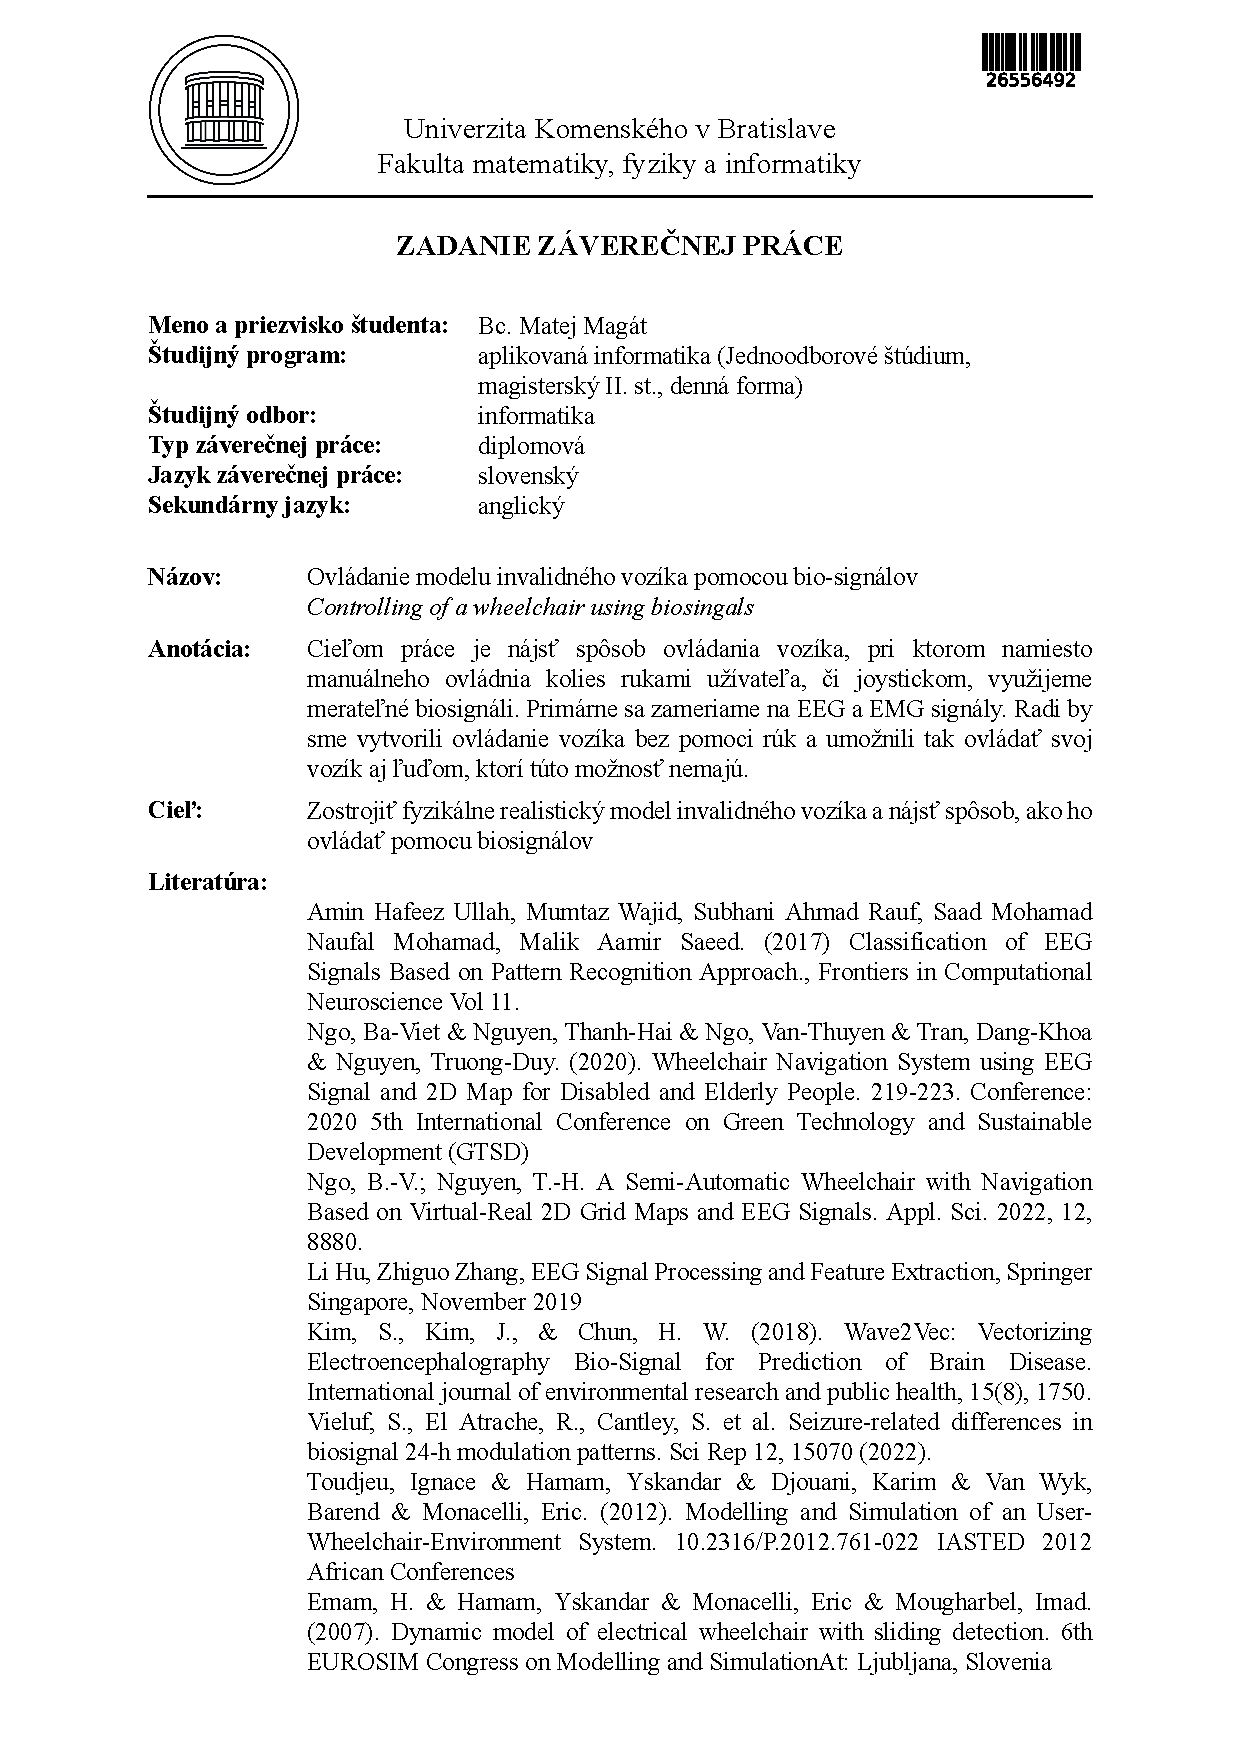
\includegraphics[width=1.0\textwidth]{images/zadanieDP}

% --- Koniec zadania

\frontmatter
\begin{center}
\end{center}
% -------------------
%   Poďakovanie - nepovinné
% -------------------
\setcounter{page}{3}
\newpage 
~

\vfill
{\bf Čestné prehlásenie:} \\
{\tab[2cm] Čestne prehlasujem, že túto diplomovú prácu som vypracoval samostatne s použitím uvedených zdrojov ... .}
\newpage 
~

\vfill
{\bf Poďakovanie:}  \\
{\tab[2cm] Chcel by som sa takouto formou poďakovať môjmu školiteľovi \mfskolitel za rady a usmernenia počas mojej práce na tejto téme ... .}
% --- Koniec poďakovania

% -------------------
%   Abstrakt - Slovensky
% -------------------
\newpage 
\section*{Abstrakt}
Magát, Matej.   \textsl{\mfnazov}
[Diplomová práca]. Univerzita Komenského v Bratislave. Fakulta matematiky, fyziky a 
informatiky; Katedra aplikovanej informatiky. Školiteľ: \mfskolitel; Konzultant: \mfkonzultant; Komisia pre obhajoby: Aplikovaná informatika. Predseda: ... stupeň 
kvalifikácie: Magister. Bratislava: FMFI UK, 2024. .\\
\newline
\tab[5 mm] Cieľom mojej diplomovej práce bolo nájsť vhodné biosignály, ktoré by sa dali použiť na ovládanie elektrického (inteligentného) vozíka a ich použitie na interakciu s počítačom, či iným elektronickým zariadením, a umožniť tak zdravotne znevýhodneným, obzvlásť ľudom, ktorý majú ochrnuté ruky ovládať elektronické zariadenia. Počas plnenia cieľa vnikol (vznikli) program na ovládanie myši ... .\\

\vfill
\paragraph*{Kľúčové slová:} biosignály, elektrický vozík, ... 
% --- Koniec Abstrakt - Slovensky


% -------------------
% --- Abstrakt - Anglicky 
% -------------------
\newpage 
\section*{Abstract}
....


\paragraph*{Keywords: biosignals, ....} 

% --- Koniec Abstrakt - Anglicky

% -------------------
% --- Predhovor - v informatike sa zvacsa nepouziva
% -------------------
%\newpage 
%\thispagestyle{empty}
%
%\huge{Predhovor}
%\normalsize
%\newline
%Predhovor je všeobecná informácia o práci, obsahuje hlavnú charakteristiku práce 
%a okolnosti jej vzniku. Autor zdôvodní výber témy, stručne informuje o cieľoch 
%a význame práce, spomenie domáci a zahraničný kontext, komu je práca určená, 
%použité metódy, stav poznania; autor stručne charakterizuje svoj prístup a svoje 
%hľadisko. 
%
% --- Koniec Predhovor


% -------------------
% --- Obsah
% -------------------

\newpage 

\tableofcontents

% ---  Koniec Obsahu

% -------------------
% --- Zoznamy tabuliek, obrázkov - nepovinne
% -------------------

%\newpage 

%\listoffigures
%\listoftables

% ---  Koniec Zoznamov

\mainmatter


\chapter*{Slovník pojmov} % chapter* je necislovana kapitola
 \addcontentsline{toc}{chapter}{Slovník pojmov} %rucne pridanie do obsahu
\markboth{Slovník pojmov}{Slovník pojmov} % vyriesenie hlaviciek
\begin{itemize}
  \item Biosignály rozumiem elektrické signály z mozgu alebo z elektrického impulzu pre sval
\end{itemize}
\chapter*{Úvod} % chapter* je necislovana kapitola
 \addcontentsline{toc}{chapter}{Úvod} %rucne pridanie do obsahu
\markboth{Úvod}{Úvod} % vyriesenie hlaviciek

{ 
\tab[5mm] V dnešnej digitálnej dobe sú tradičné ovládacie metódy, ako sú klávesnica a myš, neodmysliteľnou súčasťou našej interakcie s počítačmi. Avšak, pre niektorých jednotlivcov postihnutých rôznymi fyzickými alebo neurologickými obmedzeniami môžu tieto konvenčné prostriedky predstavovať výzvu. Je preto nevyhnutné hľadať inovatívne a prispôsobené spôsoby ovládania, aby sme zabezpečili prístup k digitálnym technológiám pre všetkých.

\tab[5mm] Táto diplomová práca sa zameriava na štúdium využitia biosignálov pri vytváraní netradičných spôsobov ovládania elektrických zariadení a následne možné ovládanie virtuálneho vozíka. Biosignály predstavujú rôznorodú paletu fyzikálnych signálov generovaných živými organizmami, ktoré možno využiť na interakciu s počítačom. V rámci tohto štúdia bude špeciálny dôraz kladený na využitie Brain-Computer Interface (BCI) ako jedného z prístupov, ktorý môže poskytnúť vhodné biosignály pre netradičné ovládacie mechanizmy.

\tab[5mm] V nasledujúcich častiach práce sa však budeme zaoberať hlavným smerom nášho výskumu, a to využitím biosignálov na ovládanie pomocou jazyka. Analyzovať budeme nielen technické aspekty tejto problematiky, ale aj aplikácie a výhody, ktoré môže ponúknuť pre jednotlivcov s obmedzeniami. Cieľom bude preskúmať a vyvinúť inovatívne metódy, ktoré umožnia efektívne a presné ovládanie počítača prostredníctvom jazyka.
}

{ 
\tab[5mm] Začínajúci výskum \cite{s16111806} a \cite{app12178880} v oblasti biomedicíny ponúka zaujímavý pohľad na možnosť interakcie medzi osobou používajúcou invalidný vozík a počítačom s využitím umelej inteligencie (AI). Tieto štúdie naznačujú, že takáto interakcia by mohla byť realizovaná v reálnom čase, čím by sa otvárali nové perspektívy pre efektívne ovládanie vozíka.

}

{
\tab[5mm] Cieľom tejto diplomovej práce je identifikovať vhodné biosignály, prípadne ich kombinácie, ktoré by mohli slúžiť ako efektívne ovládacie mechanizmy pre invalidné vozíky. Kvôli technickým obmedzeniam práce s reálnymi vozíkmi a obmedzeniam v reálnom čase sa budeme zamerať na vývoj a testovanie týchto ovládacích mechanizmov na virtuálnych prostrediach s výstupom simulovaného ovládania myšou. Týmto spôsobom sa snažíme poskytnúť užitočné poznatky a návrhy, ktoré by mohli byť v budúcnosti implementované v reálnom prostredí.
}
\chapter{Súčasný stav}

\tab[5 mm] V tejto časti práce sa budeme venovať prehľadu súčasného stavu problematiky ovládania pomocou biosignálov, so zameraním na domáce a zahraničné výskumy a implementácie, a ktoré boli počas robenia tejto diplomovej práce skúmané, poprípade uvažované. Pozrieme sa napríklad na vývoj elektroencefalografu (EEG signálov),  elektromyografického (EMG signálov), elektrokardiografického (ECG signálov) a elektrodermálneho (EDA signálov), na Brain-Computer Interface (BCI) technológie ako bitalino, neuralink, asistenčné technológie ako prístroj na ovládanie počítača pomocou očí (tobii), úst, asistenčné technológie pre nevidiacich. V tejto kapitole sa budú opisovať rôzne výhody a nevýhody daných technológii, poprípade ich riziká.


\section{História}
\tab[5 mm] Táto podkapitola poskytuje prehľad o histórii EEG, zdôrazňujúc prínosy a vývoj od jeho počiatkov, ktoré boli neoddeliteľne spojené s prácou Hansa Bergera.
\subsection{Prvé Kroky: Objav Elektrických Aktivít v Mozgu}
\tab[5 mm] V roku 1924 dosiahol Hans Berger[4*] kľúčový milník, keď prvýkrát zaznamenal elektrické aktivity v ľudskom mozgu prostredníctvom elektroencefalografu(EEG). Tento objav znamenal začiatok elektroencefalografie a poskytol nový pohľad na štúdium mozgovej činnosti.\\
\subsection{Kontinuálny Vývoj EEG Technológie}
\tab[5 mm] S postupujúcim časom sa EEG technológia neustále zdokonalovala. Výskumy a experimenty Hansa Bergera a jeho nasledovníkov pomohli vytvoriť sofistikované EEG prístroje, ktoré umožňujú detailnejšie sledovanie mozgovej aktivity.
\subsection{Prínosy Pre Medicínu a Výskum}

\tab[5 mm] Hans Bergerov výskum a jeho vynálezy v oblasti EEG mali významný vplyv na medicínsku diagnostiku a výskum mozgovej činnosti. EEG sa stal dôležitým nástrojom pri identifikácii neurologických porúch a štúdiu rôznych stavov mozgu.

\subsection{Nadväzujúci Výskum a Vývoj}
\tab[5 mm] Článok taktiež pripomína, že po Bergerových počiatkoch nasledovalo mnoho ďalších výskumníkov, ktorí prispeli k ďalšiemu rozvoju a porozumeniu EEG. Ich prínosy viedli k rôznym aplikáciám, vrátane vývoja moderných Brain-Computer Interface (BCI) technológií.


\section{Elektromyograf (EMG)}
\tab[5 mm] Elektromyografia (EMG) je diagnostická a výskumná technika, ktorá sa zaoberá meraním a analýzou elektrických signálov generovaných svalovými vláknami v tele. Táto metóda poskytuje dôležité informácie o svalovej aktivite, kontrakciách a koordinácii svalových skupín.\\
\tab[5 mm] EMG využíva elektrody umiestnené na povrchu kože alebo priamo v svaloch, ktoré zachytávajú elektrické impulzy, ktoré vznikajú pri kontrakcii svalov. Tieto impulzy sú následne zaznamenané a analyzované na získanie podrobnejších údajov o svalovej činnosti.\\
\tab[5 mm] V roku 2014 Farina, Merletti a Enoka \cite{doi:10.1152/japplphysiol.00162.2014} prezentovali významné aktualizácie v oblasti extrakcie neurálnych stratégií zo signálov povrchovej elektromyografie (sEMG). Táto štúdia vznikla v reakcii na výzvy spojené s komplexnou neurálnou kontrolou svalu a snažila sa prekonať nedostatky povrchového merania, ktoré sa ukázalo ako náchylné na interferencie a nepresné.\\
\tab[5 mm] Jedným z hlavných problémov, ktoré ovplyvňovali presnosť sEMG meraní, bolo množstvo miest, kde neuróny vstupujú do svalov, čo vytvára zložité vzory elektrických aktivít. Zistenie, že len približne 60\% týchto vzorov je možné presne odlíšiť, zdôraznilo potrebu zlepšiť metódy merania.\\
\tab[5 mm] V snahe zvýšiť presnosť sEMG meraní výskumníci experimentovali s viacerými prístupmi. Jedným z hlavných krokov bolo využitie hrubších elektród, aby sa zlepšila citlivosť a minimalizovali interferencie. Taktiež sa rozšírili na meranie elektrických aktivít v mozgu (EEG) a mieche, s cieľom získať komplexnejší pohľad na vzory centrálnej regulácie svalovej aktivity.\\
\tab[5 mm] Vzhľadom na to, že neuróny vstupujú do svalov na mnohých miestach, zabezpečilo systematické skúmanie interferencií a vývoj nových filtračných techník dôležitý prínos k presnejšiemu zachyteniu a interpretácii neurálnych vzorov.\\
\tab[5 mm] Výsledkom týchto opatrení bolo výrazné zlepšenie presnosti meraní sEMG, čo otvorilo cestu k presnejšiemu určeniu neurálnych stratégií a lepšiemu pochopeniu centrálnej regulácie svalovej aktivity. Tieto inovácie predstavujú významný krok vpred v oblasti výskumu sEMG a sľubujú rozsiahlejšie poznatky pre budúce vývojové smery [\cite{doi:10.1152/japplphysiol.00162.2014}].

\section{Domáce Prístupy}
\subsection{Popis problému}
\tab[5 mm] V kontexte Slovenska je stále vzrastajúci záujem o výskum a aplikácie Brain-Computer Interface (BCI). Práce, ako napríklad [3* - RIADENIE MOBILNÉHO ROBOTA POMOCOU EEG SIGNÁLOV MOZGU DIPLOMOVÁ PRÁCA], ďalšia praca na túto tému [5* - SNÍMANIE A SPRACOVANIE EEG SIGNÁLOV MOZGU PRE ÚČELY VYUŽITIA V SYSTÉMOCH HMI DIPLOMOVÁ PRÁCA], prispievajú k rozvoju poznatkov v oblasti BCI a jeho aplikácií v domácom prostredí.\\ 
\tab[5 mm] Obe práce sa zaoberajú konkrétnymi aspektmi vývoja a implementácie BCI technológií pre lokalizované potreby, V týchto diplomových prácach sa venovali problematike elektroencefalografie (EEG) a jej aplikáciám.

\section{popis technológií}
\subsection{Elektroencefalograf (EEG)}
\tab[5 mm] Elektroencefalograf (EEG) predstavuje nástroj navrhnutý na zaznamenávanie elektrických aktivít v mozgu. Tieto elektrické signály, generované komunikáciou medzi mozgovými neurónmi, sú zachytávané sériou malých kovových diskov, nazývaných elektrody, umiestnených na povrchu hlavy. Následne sú tieto slabé signály zosilnené pomocou preampfikátora a zaznamenávané elektronickým záznamovým systémom. EEG umožňuje sledovať charakteristické vlny mozgovej aktivity, ktoré sú následne využívané v oblasti neurologie, psychiatrie, a výskumu mozgovej činnosti. Jeho neinvazívna povaha a schopnosť poskytovať detailný pohľad na stav mozgu robia z EEG významný nástroj pre diagnostiku, monitorovanie a vedecký výskum. Na obrázku nižšie vidieť záznam z elektroencefalografu.\\
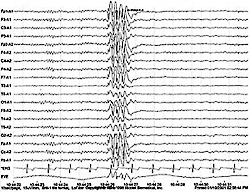
\includegraphics[width=1.0\textwidth]{images/eeg.jpg}\\
\tab[5 mm] Aby elektroencefalograf (EEG) mohol správne fungovať musíme poznať základnú topológiu ľudského mozgu a aj jeho základné funkcie aby sme mohli elektroencefalograf (EEG), Ľudský mozog, zložený z neurónov, predstavuje komplexný neuroanatomický systém, ktorý je charakterizovaný rôznymi stupňami vzájomnej prepojenosti neurónov. V tomto zmysle tvorí kôra mozgu, čo je najvonkajšia vrstva mozgového tkaniva, významnú časť tohto neuroarchitektonického usporiadania. Konkrétne, kôra mozgu obýva približne 70\% neurónovej populácie v ľudskom mozgu[3*]. \\
\tab[5 mm] Elektrický signály medzi bunkami ľudského mozgu (neurónov) vzniká v dôsledku ich polarizácie, čo je zachytávané ako elektroencefalografické (EEG) signál. Tieto aktivity môžeme merať aj na povrchu, signál je však veľmi slabí a to na úrovni desiatok mikrovoltov. Hlavnými zdrojmi elektrickej aktivity mozgu sú akčné potenciály a postsynaptické potenciály excitácie a inhibície (EPSP a IPSP)[3*].\\
\tab[5 mm] Na kôre mozgu sa vyskytujú akčné potenciály a hromadné excitácie postsynaptických potenciálov , čo je zásadným faktorom synchronizovanej aktivity EEG. Synchronizácia výbojov talamických jadier závisí na zmene ich membránového potenciálu prostredníctvom informácií z EPSP, čím sa aktivujú napäťové Ca2+ kanály a vytvára sa cyklus vedúci k akčnému potenciálu talamických neurónov[3*].\\
\tab[5 mm] Následne nasleduje hyperpolarizácia membrány, ktorá je obnovená prúdom draslíka. Cholinergné vstupy z mozgového kmeňa a predného mozgu udržiavajú membránový potenciál talamických jadier, umožňujúc prenos senzorických informácií do mozgovej kôry v aktívnom stave[3*].\\
\tab[5 mm] Ľudský mozog, s obsahom 86 miliárd neurónových buniek, zahŕňa viacvrstvovú pavučinu neurónov a rozsiahle množstvo gliových buniek, ktoré stabilizujú chemické prostredie a regulujú a chránia neuróny. Mozgová kôra, ktorá predstavuje približne 70\% všetkých neurónov mozgu, je rozdelená na štyri hlavné časti: čelový lalok, temenný lalok, záhlavný lalok a spánkový lalok, každý s špecifickými úlohami pri spracovaní informácií[3*].\\
\tab[5 mm] Neuróny sú schopné vysielať tisíce impulzov za sekundu, čím vytvárajú okruh elektrických signálov, ktoré je možné zaznamenať pomocou EEG. Signály môžu byť zaznamenané buď ako bipolárny záznam, porovnávajúci potenciály dvoch bodov na povrchu kože lebky, alebo ako unipolárny záznam, merajúci rozdiel elektrických potenciálov medzi mozgovým tkanivom a bodom s nulovým potenciálom[3*].\\
\tab[5 mm] Po získaní EEG signálov je nevyhnutné ich zosilniť a odfiltrovať, aby sa odstránil šum. Následne sú výsledky kategorizované podľa frekvencií a amplitúd rôznych vĺn, ako sú alfa, beta, gama, delta a theta vlny, ktoré majú svoje špecifické frekvencie  a funkcie:
\tab[5 mm] Gama vlny (40 - 100 Hz) sú dominantné v situáciách, kedy vystavujeme náš mozog náročným úlohám. Napríklad pri trénovaní na Menteme. Gama frekvencia hrá dôležitú úlohu pri učení a pamäti.\\
\tab[5 mm]  Beta vlny sú aktívne v bdelom stave. Nachádzajú sa v rozmedzí 12-40 Hz. Čím vyššia je ich frekvencia, tým podráždenejšími sa stávame. Ovláda nás zlosť, nervozita alebo strach. Nižšia frekvencia sa vyskytuje pri pocite únavy alebo ospalosti. Vlny beta sú viditeľné pri logicko-analytickom, teda rozumovom uvažovaní. Pri ich aktivite sa zameriavame na riešenie problémov.\\
\tab[5 mm] Alfa vlny s frekvenciou 8 - 12 Hz prevládajú pri stave uvoľnenia a odpočinku. Skrátka vždy, keď si nerobíme s ničím starosti a nezahlcujeme naše zmysly žiadnymi výraznými podnetmi. Duševná pohoda, ktorú Alfa vlny vyvolávajú, zlepšujú kvalitu spánku, učenie, zvyšuje produktivitu a dokonca našu imunitu.\\
\tab[5 mm] Aktivácia Theta vĺn (4 - 8 Hz) nastáva pri hlbokej relaxácii, meditácii a v niektorých fázach spánku. Počas týchto frekvencií dochádza ku skvalitňovaniu dlhodobej pamäti a schopnosti nachádzať neobvyklé riešenia. Vzniká väčšina vizionárskych videní. Každý jogín tiež vie, že v stave aktivácie Theta vĺn dochádza k prehĺbeniu intuície a v niektorých momentoch sa možno stretnúť so svojím vlastným nevedomím.\\
\tab[5 mm] Delta vlny s frekvenciou 1-4 Hz sa objavujú pri veľmi dôkladnej meditáciu, v stave hlbokého spánku alebo v bezvedomí. Pri týchto frekvenciách dochádza k hĺbkovej regenerácii organizmu.
[3*] [5*].
% veľmi dlhé citácie vadí to??
\section{Zahraničné Prístupy}
\subsection{neuralink}
\tab[5 mm] V kontexte zahraničia je záujem o výskum a aplikácie Brain-Computer Interface (BCI) ešte väčší ako na Slovensku. Výkum v oblasti Neuralinku, ktorý je spomenutý aj v tomto článku \cite{fiani2021examination}, prispievajú k rozvoju poznatkov v oblasti BCI a jeho aplikácií v celosvetovom obore.\\
\tab[5 mm] Firma Neuralink začala ako startupová spoločnosť zakladateľa Tesly, Elona Muska a bola zaregistrovaná v roku 2016. 
\subsection{výhody a ciele}
Neuralink \cite{fiani2021examination} ako spoločnosť má za cieľ porozumieť neuropatologickým stavom a liečiť liečiť ich.
Firma Neuralink deklaruje, že má za cieľ pomáhať jednotlivcom s rôznymi formami telesného postihnutia, umožniť
 ľudom, aby prepojili svoje mozgy so strojmi a pomocou umelej inteligencie (AI) dosiahnuť nové možnosti.
 Niektoré možnosti by mali byť pohyb exoskeletu (pripevnenom na tele pacienta) alebo inej robotiky s pomocou ich ich mysle, toto by umožnilo komunikáciu s pacientom s zdravotným postihnutým, predišlo by syndrómu uzamknutia z dôvodu neschopnosti komunikovať, čo by malo za pozitívny následok obnovenie neurónových spojení stratených pri degeneratívnych ochoreniach
 poruchy, ako je Alzheimerova choroba.\\
 \tab[5 mm] ďalšími možnosťami monitorovanie a tréning ľudských psychofyziologických stavov a
 kognitívne schopnosti a pomoc pri prevencii záchvatov a liečbe farmakorezistentnej epilepsie. k týmto cieľom vedie podľa firmy Neuralink vytvorenie rozhrania mozog-stroj (BMI), ktoré by mohlo obnoviť obe senzorické funkcie
 a motorické funkcie u jedincov s neurologickými poruchami pomocou implantovaných elektród priamo do mozgu.  tieto elektródy sú pospájané \uv{vláknami}, na ktoré sú umiestnené. Tieto elektródy možno chirurgicky implantovať do mozgu jednotlivca pomocou robota navrhnutého spoločnosťou.  Tieto elektródy poskytujú v reálnom čase údaje o aktivite vybranej skupiny neurónov s väčšou presnosťou ako elektródy na koži popísané vyššie. Údaje z neurónov sú prezentované ako vzory na rozhraní, ktoré sa dajú \uv{podhodiť} umelej inteligencie (AI), ktorej umelé neuróny spracujú signál podobne ako by to urobili skutočné neuróny.  Tieto údaje môžu byť konvertované algoritmicky a uložené v
 externé zariadenie Neuralink s možnosťou osobne sledovať tieto údaje prostredníctvom zariadenia Neuralink iPhone
 aplikácie.  Táto technológia má veľké dôsledky v oblasti neurochirurgie.  
\subsection{nevýhody}
\tab[5 mm] V článku rozoberali \cite{fiani2021examination} aj rizyká spojené s implantáciou zariadenia, ktorá vyžaduje robota aj živého neurochirurg. Zákrok vyžaduje prítomnosť oboch, pretože zámerom malej veľkosti elektródy bol prístup k anatomicky chráneným neurónom bez poškodenia susedného tkaniva. \\
\tab[5 mm] Účinnosť tohto zariadenia je tiež obmedzená špecifickými typmi patológií, s ktorými sa pacienti vyskytujú.
 Ak dôjde k poškodeniu motorickej kôry alebo miechy pri implantácii zariadenia, následná \uv{oprava} je príliš ťažká alebo so súčasnou technikou priam nemožná. Táto metóda získavania signálov z mozgu požaduje chyrurgický - invazívny zásach do nášeho najcitlivejšieho orgánu, mozgu, navyše sa tento zákrok dá spraviť len v špecializovanom zariadení, takže táto metóda z tejto diplomovej práce odpadá.  
\subsection{6DOF}
\tab[5 mm] Metóda, ktorú navrhovali v \cite{sunny2021eye} je určená pre jednotlivcov s motorickými dysfunkciami horných (a aj dolných končatín. Pre toto postihnutie ako je aj v článku povedané vykonávanie každodenných činností je pre postihnutého človeka bez pomoci druhej osoby prakticky nemožné, preto sa autori zamerali na robotickú ruku na invalidnom vozíku. Túto možnosť skúmali z hľadiska vyššieho stupňa postihnutia hornej končatiny respektíve neschopnosti ovládať invalidný vozík alebo robotické rameno pomocou iných štandardných vstupných zariadení, ako je joystick ovládaný prstom alebo bradou. V tomto článku rozoberali nimi vyvinutý riadiaci systém a rozhranie sú overené prostredníctvom experimentov so zdravými účastníkmi. Ich experimenty zahŕňali rôzne základné činnosti každodenného života a ovládanie invalidného vozíka pomocou rovnakého rozhrania, ktoré je tiež potrebné pre nezávislosť pohybu osôb so zdravotným postihnutím. \\
\tab[5 mm] V článku popisovali aj nimi navrhnuté grafické rozhranie, pričom veľký dôraz kládli na jednoduchosť a veľké ikony. Ich metóda zahŕňala pohyb očí, využívajúcu technológiu Tobii popísanú nižšie. V článku robili pokusy na 10 zdravých ľudoch, ako sami poznamenali, táto metóda sa nedá použiť na osobách trpiacich očnými vadami, preto by bolo vhodné pridať do ich softvéru detekciu objektov čím by bolo možné vymeniť oči za tvár.
\section{Hotové technológie}
\tab[5 mm] V tejto sekcii budeme rozoberať už existujúce assistenčné technológie pre ľudí s obmedzenou pohyblivosťou, s ktorými sme sa počas písania tejto diplomovej práce stretli (nebudeme tu opisovať assistenčné technológie, ktoré sú síce na svete, ale sú nápomocné pre inú kategóriu ľudí ako je DMO).
\subsection{Bitalino}
\tab[5 mm] Bitalino je revolučný biomedicínsky zberač dát, ktorý poskytuje komplexný pohľad na fyziologické parametre ľudského tela. Jeho kompaktný a ľahko prenosný dizajn umožňuje používateľom získavať bioelektrické signály a ďalšie dôležité údaje v reálnom čase, čím otvára dvere pre rozsiahlu škálu výskumu a monitorovania.\\
\tab[5 mm] S vybavením rôznymi senzormi vrátane elektromyografického (EMG), elektrokardiografického (ECG) a elektrodermálneho (EDA) senzora, Bitalino poskytuje podrobné informácie o svalovej aktivite, srdcových signáloch a elektrickej vodivosti kože. Tieto údaje majú zásadný význam pre monitorovanie zdravia, vedecký výskum a diagnostiku. Taktiež bitalino slúži na zber elektroencefalografických (EEG) signálov.\\
\tab[5 mm] Jeho jednoduchá integrácia so softvérovými platformami umožňuje užívateľom efektívne ukladať, analyzovať a zdieľať namerané dáta. Bitalino sa stáva nenahraditeľným nástrojom nielen pre profesionálnych výskumníkov v oblasti biomedicíny, ale aj pre študentov a nadšencov, ktorí chcú preskúmať a porozumieť fyziologickým aspektom ľudského tela.\\
\tab[5 mm] Jeho flexibilita, spoľahlivosť a schopnosť presného merania robia z Bitalino špičkový nástroj pre rôzne oblasti, vrátane výskumu, školského vzdelávania a monitorovania zdravotného stavu. S Bitalinom je sledovanie fyziologických parametrov jednoduché, presné a prispôsobiteľné pre rôzne potreby a aplikácie.\\
\tab[5 mm] Bitalino je taktiež schopný merať elektroencefalografických (EEG) signálov. Môže byť použitý na monitorovanie aktivity mozgu a získavanie dát o elektrických impulzoch generovaných mozgovými neurónmi.\\
\tab[5 mm] Pre EEG meranie Bitalino často využíva elektrody umiestnené na povrchu lebky, ktoré zachytávajú elektrické signály vyvolané mozgovou činnosťou. Týmto spôsobom môže poskytnúť informácie o rôznych frekvenciách mozgových vĺn, ktoré sú dôležité pre analýzu stavu mozgu, učenia, pamäti a ďalších kognitívnych funkcií. Ako už bolo skôr spomenuté vyššie signály nie sú signálmi jednotlivých neurónov, ale celých skupín (oblastí) neurónov.\\
\tab[5 mm] Je však dôležité poznamenať, že Bitalino nie je špecializovaný výlučne pre EEG merania a jeho schopnosti v tejto oblasti môžu byť obmedzené v porovnaní s profesionálnymi EEG zariadeniami.\\
\tab[5 mm] Ako sa neskôr ukázalo signály EEG je tažké z neho príjmať.  
\subsection{Tobii PCEye}
\tab[5 mm] Tobii PCEye je zariadenie navrhnuté na sledovanie pohybu očí a jeho integrovanie s počítačom pre rôzne účely, najmä pre užívateľov s obmedzenou pohyblivosťou. \\
\tab[5 mm] Tobii PCEye je vybavené technológiou sledovania pohybu očí, ktorá umožňuje presné monitorovanie, kam užívateľ pozoruje svojimi očami.\\
\tab[5 mm] Zariadenie obvykle obsahuje infračervenú kameru, ktorá sleduje polohu očí užívateľa. Táto kamera je často umiestnená pod alebo nad obrazovkou počítača.\\
\tab[5 mm] Pred použitím je potrebné vykonať kalibráciu, aby bolo zariadenie schopné presne rozpoznať pohyby očí konkrétneho užívateľa.\\
\tab[5 mm] K Tobii PCEye obvykle patrí aj špeciálny softvér, ktorý spracováva údaje z kamery a prevádza ich na akcie na obrazovke. Tento softvér môže umožňovať ovládanie kurzoru, písanie textu, navigáciu po webových stránkach alebo používanie iných aplikácií.\\
\tab[5 mm] Tobii PCEye sa často používa ako asistenčný nástroj pre ľudí s telesným postihnutím alebo inými obmedzeniami. Pomáha im komunikovať, ovládať počítač a získavať prístup k digitálnym informáciám.\\
\tab[5 mm] Zariadenie sa obvykle pripája k počítaču pomocou USB rozhrania a môže byť kompatibilné s rôznymi operačnými systémami.\\
\tab[5 mm] Tobii PCEye a podobné zariadenia prinášajú významné zlepšenia kvality života ľudí s obmedzenou pohyblivosťou, umožňujú im nezávislosť a umožňujú im plnohodnotne využívať digitálne technológie.\\
\tab[5 mm] Tobii PCEye vyžaduje špeciálny softvér na spracovanie údajov zo sledovania pohybu očí a prekladanie týchto údajov do konkrétnych akcií na počítači. Tento softvér umožňuje užívateľovi ovládať kurzor, písať text, vykonávať rôzne úlohy a interagovať s rôznymi aplikáciami pomocou pohybov očí. Bez tohto špeciálneho softvéru by bolo zariadenie Tobii PCEye nefunkčné.\\
\tab[5 mm] Je to super technológia, no ukázalo sa, že je náročná na pozornosť očí a stabilitu trupu, pre mnohé osoby so zdravotným postihnutým, ktoré majú pohyblivý trup je fyzicky náročné udržať sa v jednej pozícii.
\subsection{EVA Facial Mouse}
Na podobnom existujú aplikácie na platforme Android, ktoré využívajú sledovanie pohybu očí na interakciu s smartfónom alebo tabletom. Jednou z populárnych aplikácií tohto typu je EVA Facial Mouse. Táto aplikácia bola vyvinutá pre užívateľov s obmedzenou pohyblivosťou a umožňuje im ovládať zariadenie pomocou pohybov očí.\\
\tab[5 mm] Princíp je podobný ako pri Tobii PCEye, ale upravený pre mobilné zariadenia s dotykovými obrazovkami. Aplikácia používa prednú kameru zariadenia, ale namiesto na sledovania pohybu očí umožňuje užívateľovi ovládať kurzor, pomocou pohybu hlavy.



\newpage
\section{Programovacie jazyky}
\subsection{Python}
\subsubsection{Popis jazyka}
\tab[5 mm] Prvou možnosťou pre túto diplomovú prácu sa naskytol programovací jazyk Python, ktorý je podľa článku z decembra 2017 \cite{srinath2017python} najrýchlejšie rastúcim programovacím jazykom na svete. Python je výkonný vysokoúrovňový, objektovo orientovaný programovací jazyk vytvorený Guidom van Rossumom. Guidom van Rossumom Pracoval pre spoločnosti:\\
\tab[5 mm] Dropbox je americká technologická spoločnosť zameraná na cloudové úložisko a spoluprácu, ktorú založili Drew Houston a Arash Ferdowsi v roku 2007. Spoločnosť Dropbox poskytuje služby cloudového úložiska, ktoré umožňujú používateľom ukladať, synchronizovať a zdieľať súbory medzi rôznymi zariadeniami. Od svojho založenia sa Dropbox stal jedným z popredných poskytovateľov cloudových služieb na svete. \\
\tab[5 mm] Google je jednou z najväčších a najvplyvnejších technologických spoločností na svete, založená v roku 1998 Larrym Pageom a Sergeyem Brinom. Spoločnosť Google je známa pre svoje internetové vyhľadávanie, online reklamy, cloudové služby, mobilné technológie a mnoho ďalších inovácií. Okrem toho je Google tvorcom mnohých populárnych nástrojov a produktov, vrátane programovacieho jazyka Python, ktorý vytvoril Guido van Rossum.\\
\tab[5 mm] Elemental Security je spoločnosť zameraná na bezpečnostné riešenia, ktorá poskytuje nástroje na správu a monitorovanie bezpečnosti IT infraštruktúry. Spoločnosť sa špecializuje na poskytovanie riešení, ktoré pomáhajú organizáciám chrániť svoje siete, dáta a systémy pred kybernetickými hrozbami. Jej produktové a služobné portfólio sa sústreďuje na prevenciu a detekciu bezpečnostných hrozieb v dynamickom prostredí informačných technológií. \\
\tab[5 mm] Zope Corporation je spoločnosť so zameraním na open-source softvér a webové technológie, známa pre svoj vplyv na vývoj webových aplikácií. Zope Corporation sa podieľala na vývoji frameworku Zope, ktorý umožňuje vytváranie komplexných webových aplikácií a správu obsahu. Jej príspevky k open-source komunite zahŕňajú nástroje, ktoré uľahčujú vývoj a správu obsahu pre webové stránky a aplikácie. \\
\tab[5 mm] BeOpen.com bola spoločnosť, ktorá sa zaoberala podporou a vývojom open-source softvéru a inovatívnymi riešeniami v oblasti IT. Spoločnosť BeOpen.com podporovala mnohé projekty v open-source komunite a vytvorila platformy na podporu spolupráce a vývoja voľne dostupného softvéru. Jej angažovanosť v open-source prispela k rozvoju a šíreniu mnohých populárnych technologických nástrojov a projektov. \\
\tab[5 mm] CNRI (Corporation for National Research Initiatives) je organizácia zameraná na výskum a vývoj v oblasti informačných technológií so sídlom v USA. Organizácia sa venuje rôznym projektom a iniciatívam, ktoré smerujú k posilneniu informačných technológií a ich vplyvu na spoločnosť. CNRI podporuje aj vývoj a šírenie open-source technológií a má významné miesto v oblasti informačných štúdií.\\
\tab[5 mm] CWI (Centrum Wiskunde and Informatica) je holandský výskumný ústav v oblasti matematiky a informatiky, ktorý sa zameriava na vedu a výskum v týchto disciplínach. V rámci svojich aktivít CWI prispel k rozvoju viacerých významných technologických inovácií a projektov v oblasti informatiky.\\
\tab[5 mm] SARA (Stichting Academisch Rekencentrum Amsterdam) je akademické výpočtové centrum so sídlom v Amsterdame, ktoré poskytuje výpočtové zdroje a podporu výskumu a vzdelávaniu. Centrum SARA sa angažuje v poskytovaní výpočtových infraštruktúr pre vedecké projekty a spolupracuje s rôznymi akademickými a výskumnými organizáciami.   Jeho úloha v poskytovaní výpočtových služieb je kľúčová pre podporu vedeckého výskumu v Holandsku. \\ 
Python vytvoril počas jeho práce v CWI\cite{PYthon5}. Python podporuje veľa programovacích paradigiem, vrátane objektovo orientovaného, imperatívneho, funkcionálneho alebo procedurálneho štýlu, pričom všetko v Pythone je objekt. Objektovo orientované programovanie (OOP) vám pomáha intuitívne riešiť komplexné problémy. S OOP môžete tieto zložité problémy rozdeliť na menšie sady vytváraním objektov.
Python je viacparadigmový programovací jazyk, ktorý plne podporuje objektovo orientované programovanie a štruktúrované programovanie. Programovací jazyk Python používa dynamické typovanie a kombináciu počítania referencií a detektora cyklov pre riadenie pamäti. \\
\tab[5 mm] Existuje Programovací jazyk Python verzia 2 a Programovací jazyk Python verzia 3, verzia 2 bola staršia a dnes sa už nepoužíva - je zastaralá, preto, v tejto diplomovej práci Programovací jazyk Python bude znamenať verziu 3.  
Programovací jazyk Python bol navrhnutý tak, aby bol vysokej mierky rozšíriteľný. Programovací jazyk Python je možné tiež vložiť do existujúcich aplikácií, ktoré potrebujú programovateľné rozhranie. Programovací jazyk Python má veľkú štandardnú knižnicu, ktorá poskytujúc nástroje vhodné pre mnohé úlohy, sa často prezýva ako jedna z jeho najväčších síl. Programovací jazyk Python poskytuke mimo iné aj nástroje pre internetové aplikácie ako sú podporované rôzne štandardné formáty a protokoly (ako MIME a HTTP), štandardné knižnice v Pythone sú dobre testované a používané stovkami ľudí. Medzi moduly na vytváranie grafických užívateľských rozhraní, pripájanie sa k relačným databázam, generovanie pseudonáhodných čísel, aritmetika s desatinnou presnosťou, manipulácia s pravidelnými výrazmi a jednotkové testovanie patrí tiež do výbavy tohto jazyka. Programovací jazyk Python je možné použiť na písanie širokej škály programov. Programovací jazyk Python podporuje dynamický typový systém a v základe nemá typový systém, čo môže byť pre programátora aj nevýhoda, automatický manažment pamäte s garbage collector-om, takže sa programátor nemusí starať o správu pamäte. Skripty napísané v programovacom jazyku Python môžu byť, vďaka tomu, že programovací jazyk Python je interpreter, čo znamená, že je vyhodnocovaný programom za behu samotného programu. Programovací jazyk Python má širokú podporu a beží na rôznych operačných systémoch ako sú Windows, Linux, UNIX, Amigo, Mac OS, Android a mnoho daľších. Programy napísané v programovacom jazyku Python Môžete presúvať z jednej platformy na druhú a spúšťať ich bez akejkoľvek zmeny.\\
Programovací jazyk Python sa využíva vo veľa svetových firmách uvediem niektoré z nich:\\
\tab[5 mm] Google, globálna technologická spoločnosť, využíva Python pre širokú škálu úloh, od webového vývoja po spracovanie údajov a automatizáciu.\\
\tab[5 mm] YouTube, populárna platforma na zdieľanie videí, využíva Python na spracovanie dát, analýzu obsahu a optimalizáciu svojich služieb.\\
\tab[5 mm] Populárny BitTorrent je známa platforma pre peer-to-peer sťahovanie súborov, využíva Python na rôzne účely vrátane riadenia a optimalizácie komunikácie medzi užívateľmi.\\
\tab[5 mm] ESRI, vedúca spoločnosť v oblasti geografických informačných systémov (GIS), používa Python pre vývoj a rozšírenie svojich produktov.\\
\tab[5 mm] NASA využíva Python v rámci svojich vesmírnych programov pre analýzu dát, simulácie a rôzne úlohy v oblasti výskumu a vývoja.\\
\tab[5 mm] Los Alamos National Laboratory, zameraný na výskum a vývoj v oblasti nukleárnej fyziky, využíva Python pre rôzne výpočtové úlohy a analýzu údajov.\\
\tab[5 mm] Fermi National Accelerator Laboratory, zaoberajúci sa výskumom v oblasti častice fyziky, využíva Python pre spracovanie dát a simulácie experimentov.\\
\tab[5 mm] JPL (Jet Propulsion Laboratory): JPL, súčasť NASA, používa Python pre riadenie vesmírnych misií, analýzu údajov a vývoj softvéru pre vesmírne aplikácie.\\
\tab[5 mm] iRobot, spoločnosť zameraná na vývoj robotov a automatizovaných zariadení, využíva Python pre rôzne aspekty ich softvérových riešení.\\
\tab[5 mm] Intel, Cisco, Hewlett-Packard, Seagate, Qualcomm a IBM sú popredné technologické spoločnosti, ktoré využívajú Python pre testovanie hardvéru, čo zahŕňa verifikáciu výkonu, testovanie spoľahlivosti a ďalšie aspekty hardvérového vývoja.
A mnohé daľšie tento jazyk využívajú na najrôznejšie účely.  
\cite{srinath2017python}. \\
\tab[5 mm] Programovací jazyk Python má štandartný nástroj \uv{pip}, ktorý je eodmysliteľným nástrojom pre správu balíkov v ekosystéme programovacieho jazyka Pythonu a prispieva k jednoduchosti a efektivite v ramci tohto jazyka. Nástroj \uv{pip} je štandardný správca balíkov pre programovací jazyk Python. Je to nástroj na inštaláciu, aktualizáciu a odstraňovanie balíkov (kníh, knižníc, modulov atď.) v programovacom jazyku Python. Jeho hlavnou úlohou je uľahčiť správu externých knižníc, ktoré môžu byť v Pythone používané pre rôzne projekty. \\
\tab[5 mm] Tu sú rozpísané niektoré funkcie a aspekty nástroja \uv{pip}: \\
\tab[5 mm] Nástroj \uv{pip} umožňuje jednoduchú inštaláciu externých balíkov z oficiálnych repozitárov PyPI (Python Package Index) alebo iných zdrojov. Napríklad, na inštaláciu balíka (package) \uv{requests}, stačí spustiť príkaz: \uv{pip install requests<package>.}\\
\tab[5 mm] Nástroj \uv{pip} umožňuje rýchlu aktualizáciu inštalovaných balíkov na najnovšiu verziu. Príkaz \uv{pip install --upgrade <package>} sa používa na aktualizáciu konkrétneho balíka.\\
\tab[5 mm] Príkaz \uv{pip list} zobrazuje zoznam všetkých nainštalovaných balíkov vrátane ich verzií.\\
\tab[5 mm] S pomocou \uv{pip search <keyword>} môžete vyhľadávať balíky podľa kľúčových slov. To pomáha pri objavovaní dostupných balíkov na PyPI.\\
\tab[5 mm] Na odinštalovanie balíka sa používa príkaz \uv{pip uninstall <package>}. Tým sa odstráni daný balík a jeho závislosti.\\
\tab[5 mm] Nástroj \uv{pip} môže nainštalovať všetky balíky uvedené v súbore s požiadavkami (requirements.txt). Príkaz \uv{pip install -r requirements.txt} inštaluje všetky balíky uvedené v tomto súbore.\\
\tab[5 mm] Nástroj \uv{pip} spolu s nástrojom virtualenv (ktorý je popísaný nižšie) umožňuje vytváranie a používanie virtuálnych prostredí. Tieto prostredia izolujú inštalované balíky pre konkrétny projekt.\\
\tab[5 mm] Programovací jazyk Python má aj širokú podporu pomocných programov vlastných aj nástrojov/programov z tretých strán:\\
\tab[5 mm] Nástroje virtualenv a venv, tieto nástroje umožňujú vytváranie a správu virtuálnych prostredí v jazyka Python, čo umožňuje izolovať balíky pre rôzne projekty a zabezpečuje konzistentné prostredie pre vývoj.\\
\tab[5 mm] Vývojové prostredia (IDE) PyCharm od jetbrains, VS Code a Jupyter, ktoré poskytujú pohodlné prostredie pre písanie, ladenie a správu projektov v Pythone. Každé z nich má svoje jedinečné vlastnosti a výhody.\\
\tab[5 mm] Knižnice NumPy a SciPy poskytujú výkonné a efektívne nástroje pre prácu s vedeckými a numerickými výpočtami. Sú nevyhnutné pre riešenie komplexných matematických úloh a analýzu dát.\\
\tab[5 mm] Pandas je knižnica na analýzu dát, ktorá umožňuje efektívne manipulovať s tabuľkovými dátami a vykonávať rôzne operácie na dátových rámcov.\\
\tab[5 mm] Pytest je nástroj na testovanie v jazyku Python, ktorý ponúka jednoduchú syntax a bohaté funkcie pre písanie a spúšťanie testov.\\
\tab[5 mm] TensorFlow a PyTorch sú knižnice pre strojové učenie a hlboké učenie. Poskytujú nástroje na vytváranie, trénovanie a nasadenie modelov umelých neurónových sietí.\\
\tab[5 mm] Cython predstavuje výkonný nástroj pre programátorov, ktorí potrebujú kombinovať výhody Pythonu s výkonom jazyka C. S jeho pomocou môžeme dosiahnuť optimalizovaný kód, integrovať C knižnice a výrazne zvýšiť výkon kritických častí aplikácií. Jeho flexibilita a možnosti vytvárania rozšírení robia z Cythonu dôležitý nástroj pre vývojárov v oblasti vedeckého výskumu, výpočtovej grafiky a ďalších oblastí, kde je potrebná vysoká výkonnosť.
\newline
\newline
\tab[5 mm] Tieto nástroje spolu s mnohými ďalšími tvoria ekosystém jazyka Python, ktorý podporuje rýchly, efektívny a rozsiahly vývoj v rôznych odvetviach.

\subsubsection{Dôvody prečo si vybrať}
\tab[5 mm] Programovací jazyk Python predstavuje výnimočnú voľbu pre našu diplomovú prácu z niekoľkých dôležitých dôvodov. Python je etablovaný programovací jazyk, ktorý sa vyznačuje svojou všeobecnosťou, jednoduchosťou a širokým spektrom využitia. V nasledujúcich odsekoch uvádzame niektoré z hlavných dôvodov, prečo sme sa rozhodli práve pre tento jazyk.\\
\tab[5 mm] Programovací jazyk Python je známy svojou univerzálnosťou, ktorá umožňuje pohodlné písanie kódu pre rôzne oblasti vývoja. Je možné ho využívať od jednoduchých skriptov až po komplexné aplikácie. Táto schopnosť ho činí ideálnym nástrojom pre náš projekt, ktorý si vyžaduje rôznorodosť v rámci programovania. Pokiaľ ide o prenositeľnosť, tento je platformovo nezávislý, čo znamená, že vyvinutý kód môže bez problémov bežať na rôznych operačných systémoch, vrátane Windows, Linuxu a macOS. Táto vlastnosť zabezpečuje, že naša aplikácia bude fungovať konzistentne a bez problémov bez ohľadu na operačný systém používateľa.\\
\tab[5 mm] Programovací jazyk Python disponuje bohatou štandardnou knižnicou, ktorá poskytuje množstvo nástrojov a funkcií na riešenie bežných úloh. Tieto knižnice sú dobre testované a široko používané, čo znamená, že môžeme efektívne využívať existujúce prostriedky bez potreby opakovaného písania kódu.\\
\tab[5 mm] Programovací jazyk Python je plne objektovo orientovaný jazyk, čo znamená, že všetko v ňom je objekt. Táto vlastnosť uľahčuje prácu s komplexnými problémami, keďže umožňuje rozdelenie problému na menšie časti prostredníctvom tvorby objektov. Okrem toho podporuje multi-paradigmový prístup, čo znamená, že podporuje nielen objektovo orientované programovanie, ale aj štruktúrované programovanie. To nám dáva flexibilitu a možnosť výberu najvhodnejšieho prístupu podľa konkrétnych požiadaviek našej práce.\\
\tab[5 mm] Programovací jazyk Python má aktívnu a rozsiahlu komunitu programátorov, ktorí prispievajú k jeho neustálemu rozvoju a vylepšovaniu. Táto komunita znamená, že môžeme rýchlo získať pomoc, riešenia problémov a zdieľať skúsenosti s ostatnými vývojármi. Okrem toho existuje veľké množstvo ľahko dostupných knižníc tretích strán, čo nám umožňuje rýchlo a efektívne rozširovať funkcionalitu našej aplikácie.Celkovo vzaté, tento je pre náš projekt optimálnou voľbou vzhľadom na jeho všeobecnosť, prenositeľnosť a podporu rozsiahlej komunity.
\subsubsection{GUI jazyka Python}
\tab[5 mm] V tejto časti sa budeme zaoberať grafickými knižnicami v rámci programátorského jazyka Golang, s ktorými sme sa pri písaný tejto diplomovej práce stretli.

\subsubsection{ Tkinter}
\tab[5 mm] Tkinter je štandardná knižnica pre tvorbu GUI v jazyku Python. Poskytuje jednoduché nástroje pre vytváranie okien, tlačidiel, vstupných polí a ďalších komponentov GUI. Implementácia dostupná na \cite{PYthon6}. Je to super knižnica, ale na naplnenie cieľov sa nehodila.
\subsubsection{PyQt}
\tab[5 mm] PyQt je viazaný na Qt framework a ponúka bohaté možnosti pre tvorbu pokročilých GUI aplikácií. Obsahuje širokú škálu funkcií a nástrojov pre grafické rozhrania. Jedna verzia dostupná na \cite{PYthon7}. Táto knižnica je však málo podporovaná a roztrieštená na viacero verzii, preto sa na túto diplomovú prácu nehodila. 
\subsubsection{Kivy}
\tab[5 mm] Kivy je open-source Pythonová knižnica a framework určený na vývoj multi-touch aplikácií. Je navrhnutý tak, aby umožnil rýchly a jednoduchý vývoj pre rôzne platformy vrátane Windows, macOS, Linux, Android a iOS. Kivy podporuje tvorbu aplikácií s grafickým používateľským rozhraním, čo ho robí vhodným pre vytváranie hier, edukačných aplikácií a ďalších interaktívnych programov. \\
\tab[5 mm] Táto knižnica má schopnosť poskytovať kód, ktorý je pomerne jednoduchý pre portovanie medzi rôznymi platformami, čo uľahčuje tvorbu aplikácií pre viacero operačných systémov. Kedže táto knižnica je pod licenciou MIT, čo znamená, že je dostupný zdarma a programátori môžu prispievať k jeho vývoju, tak ju môžem použiť bez obmedzenia. \\
\tab[5 mm] Kivy poskytuje nástroje na vytváranie animácií a vizuálnych efektov, čo umožňuje vývojárom vytvárať atraktívne a interaktívne používateľské rozhrania. A preto lahko sa v nej urobí virtuálne prostredie pre skúšobnú aplikáciu.\\
\tab[5 mm] Kivy je navrhnutý s modulárnou architektúrou, čo umožňuje programátorom pridávať a odstraňovať funkcie podľa potreby. Táto vlastnosť uľahčuje rozšírenie a prispôsobenie frameworku. Táto vlastnosť sa bude hodiť ked budem chcieť rozšísiť aplikáciu o nové platformy, než tú, na ktorej to budem vyvýjať. Dostupné na \cite{PYthon9}. Preto bude Táto knižnica hlavnou grafickou knižnicou tejto diplomovej práce.

\newpage
\subsection{Golang}
\subsubsection{Popis jazyka}
\tab[5 mm] Na tvorbu diplomovej práce sme si mohli vybrať programovací jazyk Go, ktorý sa taktiež nazýva Golang, ktorý je dostupný na \cite{GOlang7}, ale len ako . možnosť.
Golang je relatívne nový jazyk, ktorý vnikol vo firme Google Inc. v roku 2007, ale jeho prvé uplatnenie nastalo 
až o dva roky neskôr desiateho novembra v roku 2009 ako je uvedené \cite{GOlang8}.\\
\tab[5 mm] Prvá verzia jazyka Golang bola vytvorená skupinou tvorenou známymi osobnosťami ako Rob Pike, ktorý je 
predovšetkým známi prácou v Bellových laboratóriách, kde bol členom tímu Unix, 
podieľal sa na tvorbe Plan 9 z operačných systémov Bellových Laboratórií a operačného systému Inferno, 
participoval na vytvorení programovacieho jazyka Limbo a je spoluautorom veľmi známeho a rozšíreného kódovania UTF-8 \cite{GOlang9},\\
Robert Griesemer, ktorý predtým pracoval na technológii JavaScript V8 spoločnosti Google, jazyku Sawzall, virtuálnom stroji Java HotSpot a systéme Strongtalk \cite{GOlang10} \\
a Ken Thompson, ktorý je skutočným velikánom v informatickej oblasti, najmä vďaka prácami
v Bellových Laboratóriách na mnohých projektoch ako napríklad operačný systém Plan 9, 
spolupráca s Robertom Pike-om na kódovaní UTF-8, operačný systém Inferno, veľmi známou a 
fundamentálnou utilitou "grep", vývojom progromovacieho jazyka B, ktorý bol predchodcom 
najrozšírenejšieho jazyka na svete (programovacieho jazyka C), podieľal sa na vývoji Belle, šachového počítača. 
Ken Thompson tiež napísal programy pre vytvorenie absolútneho hodnotenia 
(výhra, remíza alebo prehra hráča, ktorý je na ťahu) šachových postavení \cite{GOlang11}.\\
\tab[5 mm] Programovací jazyk Golang je rýchlo sa rozvíjajúcim jazykom, od jeho vydania do napísania 
tejto diplomovej práce vyšlo 21 verzií . Syntax a stavba programovacieho jazyka Golang boli inšpirované jazykmi ako sú C, Modula, Pascal a Smalltalk. \\ 
\tab[5 mm] Golang je navrhnutý tak aby sa v ňom dali písať rozličné paradigmy, medzi známe paradigmy sa zaradujú Object Oriented, aj keď mnohý kritici poukazujkú na to, že sa v Go nedá objektovo programovať (namiesto tried sa kód môže štruktúrovať pomocou package-ov), imperatíne programovanie a Vďaka svojej natívnej podpore konkurencie aj najznámejšou a najvýraznejšou paradigmou programovacieho jazyka Golang je Concurrent programming \cite{GOlang12}. \\
\tab[5 mm] Samotný programovací jazyk má jednu hlavnú a tri vedľajšie implementácie (kompilátory). 
Väčšina kompilátorov pre Golang podporuje "natívne" prepájanie (cez takzvané rozhranie cgo) a kompiláciu programovacích jazykov Golang a starého C.\\
\tab[5 mm] Hlavná implementácia je pomenovaný ako gc je to oficiálny kompilátor go-komunity,
prekladá (kompiluje) kód napísaní v jazyku Golang priamo do strojového (binárneho) kódu, ktorý 
je už plne spustiteľný, tento kompilátor síce podporuje prepájanie programovacích jazykov Golang a starého C, ale musí byť previazaný s kompilátorom, ktorý skompilujte C-éčkovskú čast kódu a komunikácia medzi nimi je časovo náročná, preto sa odporúča iba v prípade nutnosti. Tento kompilátor kompiluje veľmi rýchlo(v našich prípadoch mu trvá skompilovať program o 3600 riadkoch za 2 sekundy, binárny kód od tohto kompilátora obsahuje všetku binárnu informáciu vrátane debuggovacích nástrojov a celého runtime, preto je oproti iným binárnym kódom pomerne veľký.\\ 
\tab[5 mm] Programovací jazyk Golang má aj vedľajšie implementácie (kompilátory) sú to napríklad gccgo [13] a tiny-go [14] .\\
\tab[5 mm] gccgo je implementácia (kompilátor), ktorý je front-end kompilátora gcc, ktorý je kompilátor pre programovací jazyk C, na rozdiel od oficiálneho kompilátora gc, ktorý kompiluje priamo do binárnej podoby kompilátor gccgo najprv preloží kód písaný v programovacom jazyku Golang do programátorského jazyka C a až ten skompilujte do strojového jazyka (binárnej podoby), ďalšou odlišnosťou od oficiálneho kompilátora je v odlišnom prístupe k systémovým knižniciam respektíve k linkovaniu na nich, kým oficiálny kompilátor nepoužíva zdielané a dynamicky linkované knižnice (shared, dynamic linked library) kompilátor gccgo ich používa, tým dosahuje výrazne menší binárny kód, ale za cenu menšej prevoditeľnosti medzi jednotlivými počítačmi (musí mať všetky knižnice), ďalšou výhodou je, že má lepšie zvládnuté previazanie jazykov C a Golang (menšie časové nároky), najväčšou nevýhodou oproti štandardnému kompilátoru je, že má väčšie časové nároky na kompiláciu. \\
\tab[5 mm] Ostatné kompilátory sme nepoužívali, preto len v krátkosti opíšeme jeden, ktorý sa nám zdal najzaujímavejší. \\
Tiny-go je kompilátor, ktorý si dáva za úlohu skompilovať kód napísaný v programátorskom jazyku Golang do menšej formy vhodný pre mikročipy a mikro-počítače.\\ 
\tab[5 mm] Golang poskytuje množstvo nástrojov, ktoré sa volajú príkazom \uv{go [príkaz]}. Pri našej práci sme sa stretli s týmito:  \uv{get}, ktorý je
fundamentálny nástroj jazyka, tento nástroj slúži najmä na získavanie knižníc tretích strán. \\
Nástroj gomobile \cite{GOlang15} spolu s niektorými knižnicami sa v budúcnosti môže použiť na rozšírenie tohto programu na platformy ako Android, či IOS, tento
nástroj poskytuje dve voľby, voľbu natívneho previazania s NDK (build) alebo voľbu priviazanie (bind) s programovacími jazykmi Java (Android) a Objective-C (IOS). \cite{GOlang16} ďalšie nástroje sú napríklad godoc, ktorý sa snaží byť ekvivalentom nástroja jazyka javadoc, nástroje cover na analýzu kódu a testov, \uv{guru} a \uv{vet}.  
\subsubsection{Dôvody prečo si vybrať}
\tab[5 mm] Programovací jazyk Golang sme by sme si mohli vybrať, pretože je to síce nový jazyk, ale so zaujímavým pozadím, v ktorom sa pomerne jednoducho(a hlavne natívne) píšu konkurentné procesy, Golang poskytuje(v natívnej forme) takzvané goroutiny,  ktoré v jazyku vystupujú v roly odľahčených threadov. V našej práci by sme mohli potrebovať mať veľa paralelných(súčasne bežiacich procesov), a preto by bol programovací jazyk Golang pre našu prácu vhodným jazykom. Tento jazyk produkuje binárny kód, ktorý nepotrebuje žiadne virtuálne prostredia a v prípade klasického kompilátora(gc) ani systémové knižnice, navyše je prenositeľný na rôzne hardvérové platformy ako sú napríklad architektúry arm32, arm64, i386, amd32, amd64 a mnohé ďalšie, ale hlavne Golang je prenositeľný softvérové platformy okrem operačného systému Windows sa jeho kód môže skompilovať aj na operačné systémy Linux, Darwin(na ktorý nadväzujú systémy macOS, iOS, watchOS, tvOS a iPadOS), aix, dragonfly, android a ďalšie. Tento jazyk sme si vybrali aj vďaka jeho rýchlosti pri behu programu, ktorá sa približuje k rýchlosti vykonávania programovacieho jazyka C, ľahkej písateľnosti a čitateľnosti kódu a na koniec aj veľkému výberu ľahko dostupných knižníc tretích strán, ktoré sa automaticky stiahnu so všetkými závislosťami.
\subsubsection{GUI jazyka Golang}
\tab[5 mm] V tejto časti sa budeme zaoberať grafickými knižnicami v rámci programátorského jazyka Golang, s ktorými sme sa pri písaný tejto diplomovej práce stretli.
\subsubsection{Fyne.io/fyne}
\tab[5 mm] Táto programátorská knižnica je veľmi vyspelá a je to knižnica, ktorú podporujú aj autori pôvodného jazyka. Ako je uvedené na ich hlavnej stránke\cite{GOlang5}, tak táto knižnica je multi-platformová. Knižnica používa kompilátory gc a C-éckový gcc, ktorý musí byť 64 bitový. 
\subsubsection{gioui/gio}
\tab[5 mm] Táto programátorská knižnica je veľmi vyspelá a je to knižnica. Ako je uvedené na ich hlavnej stránke[18], tak táto knižnica je multi-platformová. Knižnica navyše pre operačné systémy Windows, Linux a Mac na štandartných platformách používa iba kód napísaný v Golang. Knižnica sa dá spustiť aj na menej využívaných platformách ako napríklad Linux  pre mobilné zariadenia alebo FreeBSD, OpenBSD, hoci tam už využíva kompilátor gcc. výhodou tejto knižnice je, že sa dá podľa[18] skompilovať(bez úprav samotného kódu) aj pre mobilné zariadenia s operačnými systémami Android a IOS/tvOS, to sa však nezaobíde bez externých nástrojov pre dané systémy. Hoci je táto vlastnosť ešte len v experimentálnej fáze najväčšou zaujímavosťou tejto knižnice je, že jej autor ju vymyslel tak, že sa dá skompilovať do Webassembléru, ktorý sa stal akýmsi novým štandardom pre internetové aplikácie.
\subsubsection{Gen2brain/raylib-go }
\tab[5 mm] Táto programátorská knižnica má výhodu, že využíva už vyladenú C knižnicu zvanú raylib, síce využíva rozhranie cgo je veľmi rýchla a istú dobu bola hlavnou knižnicou pre prvý prototyp. 
\subsubsection{Gonutz/prototype}
\tab[5 mm] Hlavnou výhodou tejto knižnice je jednoduchý interface, ktorý sa naozaj riadi heslom v jednoduchosti je krása, napriek tomu je veľmi výkonná knižnica a to aj oproti iným, ďalšou veľmi dôležitou výhodou je to, že je celá napísaná v programovacom jazyku Golang a tým zabezpečuje aj ľahšiu kompiláciu oproti iným knižniciam. Bola optimalizovaná na procesorovou architektúru Amd na operačné systémy Windows, Linux a aj Mac. Knižnica má však aj nevýhody, jednou z najväčších je to, že kód je menej prenositeľný na iné platformy ako v prípade knižnice gioui/gio, nefunguje pri nej nástroj gomobile a táto knižnica je napísaná tak, že má malý potenciál aby dosiahla preložiteľnosť na mobilné zariadenia s ich operačnými systémy (Android a IOS), nepôjde ani na vyššie uvedených operačných systémoch s inými procesorovými architektúrami, napríklad na Linuxe bežiacom na procesorovej architektúre Arm.

\section{Platforma}
\tab[5 mm] Hlavná platforma pre túto diplomovú prácu bol Linux, distribúcia Pop OS, ktorý beží na architektúre amd.
\chapter{Cieľ práce}
\tab [5 mm] Cieľom tejto diplomovej práce je nájsť vhodné biosignály (vhodné vstupy) pre ľudí s obmedzenou pohyblivosťou, aby mohli ovládať virtuálny vozík, poprípade kurzor myši od počítačového zariadenia. \\
\tab[5 mm] Na svete existuje veľmi veľa alternatív ku klasickým perifériám počítača a aj veľmi veľa spôsobov ako ovládať invalidný vozík, cieľom tejto diplomovej práce je nájsť vhodné už existujúce technológie a pokúsiť sa zlepšiť ich spolahlivosť a/alebo zvýšiť ich rýchlosť, poprípade pokúsiť sa zvečšiť ich dostupnosť, pretože u týchto technológií existujú limitujúce faktori ako je cena, presnosť a rýchlosť, práve na tieto sa v tejto diplomovej práci zameriam.\\
\tab[5 mm] Posledným cieľom bude aby výsledný program bol ľahko prenositeľný na iné platformy, než tej, na ktorej softvér bol vyvynutý.
\chapter{návrh, výskum a postup}

\section{Ovládanie kurzora programom}
\tab[5 mm] Prvý cieľ, prenositeľnosť, sa podarilo u tohto prvého myľníka splniť výberom programovacích jazykov Python a Golang.
\subsection{Popis programu}
\tab[5 mm] Tento jednoduchý program má za úlohu \uv{iba} hýbať myšou pomocou klávesníc na klávesnici podľa preddefinovaného konfiguračného súbora. Tento jednodochý program je síce vytvorený v Golangu, ale dá sa pomerne ľahko integrovať do väčšieho projektu, ktorého programovacím jazykom je Python.
\subsection{Dôvod jeho vytvorenia}
\tab[5 mm] Súčasťou tejto diplomovej práce je aj hľadať alternatívne spôsoby riadenia počítačového zariadenia, preto bolo vhodné začať práve s týmto programom.
\section{Bitalino} 
\tab[5 mm] Do tohto zariadenia sme vkladali veľké očakávania, vzhľadom na jeho písané vlastnosti, no nepodarilo sa nám z neho získať zmysluplné dáte, čo súvisí aj s povahou DMO.
\subsection{Pokus}
\tab[5 mm] Bitalino bola naša prvá voľba, kvôli potenciálu, ktorý sľuboval. Pokúsili sme sa umiestniť elektródy, podľa návodov dokumentácie k tomuto zariadeniu.  a očakávali sme ...
\subsection{Problém}
\tab[5 mm] Kvôli zášklbom sa tažko pripevňovali elektródy na svoje miesta, navyše umiestnenie ako je na obr.\\
pridať obr. .......\\
sa len tažko dosahuje aj bez zášklbov, sme usúdili, že takéto zášklby by museli mať nejaké protiopatrenia (nehovoriac o tom, že aj v mozgu by ..., ale to by sa dalo odstrániť filtrami),%, rozpitvať to v diskusii?)
 preto sme sa rozhodli preskúmať iné technológie. 
\section{Vlastné riešenie(zariadenie)} % dať samostatnú kapitolu
\tab[5 mm] Pri preskúmaní technológii ako \uv{Tobii}, \uv{Eva faciál mouse} sa nám naskytla otázka, či tieto technológie by sa dali, zrýchliť a sprístupniť, pretože \uv{Tobii} je stredne nákladná technológia, ktorá nie vždy je voľná na predaj, navyše vyžaduje  veľkú pozornosť očí. % dopísať skúsenosti, pomalé, bolia oči, nemožnosť sa pohnúť ...
\\ 
\tab[5 mm] \uv{Eva faciál mouse} je síce voľne prístupná aplikácia pre všetky android zariadenia, ale je nepresná a pomalá.\\ 
\tab[5 mm] Preto sme si povedali, že urobíme program, ktorý skombinuje rozpoznávanie tváre podobné \uv{Eva faciál mouse} a joystickom, ktorý bude ovládaný jazykom a bude sa dávať do úst.\\ 
\tab[5 mm] preto sme zvolili využitie platformy Arduino, Bluetooth modulu a joysticku. Arduino, open-source mikrokontrolér, pktorý oskytuje flexibilitu a možnosť prispôsobenia pre rôzne projekty. Jeho schopnosť interakcie s rôznymi senzormi a aktuátormi umožňuje vytvárať robustné a prispôsobiteľné asistenčné riešenia.\\ 
\tab[5 mm] Bluetooth modul je kľúčovým komponentom nášho systému, umožňujúcim bezdrôtovú komunikáciu medzi Arduino a ďalšími zariadeniami. To nám poskytne väčšiu voľnosť pohybu a umožňuje vzdialené ovládanie asistenčných funkcií.\\ 
\tab[5 mm] Joystick, ako vstupný zariadenie, bude hrať kľúčovú úlohu pri poskytovaní presného ovládania, čo následne budeme kombinovať s algoritmami počítačového videnia. Joystick bude pripevnený na držadle, do kttorého sa zahryznú zuby. \\ 
\tab[5 mm] dopísať ......
\chapter{Implementácia}
\tab[5 mm] Toto budem písať na koniec .....
\chapter{výsledky}

\chapter{Používateľské príručky}
\tab[5 mm] Tu sú popísané jednotlivé príručky k jednotlivým verziám.
\section{ Klávesnica - myš }
\tab[5 mm] 
Toto je softvér, ktorý má za cieľ umožniť ovládanie myši pomocou klávesnice. V priečinku \uv{bin} sa nachádza skompilovaný binárny súbor pre Linux a Windows (malo by byť možné spustiť aj na Macu, ale nemám Mac). V priečinku \uv{bin} je nastavenie pre Windows a v pobočke \uv{master} je nastavenie pre Linux. Ak program nenájde nastavenia, môžete ich sami prispôsobiť. V nastaveniach sú: 
\begin{itemize}
\item	Šípky na ovládanie pohybu myši
\item	 \uv{Enter},  pre ľavé kliknutie myšou 
\item	\uv{Delete}, pre pravé kliknutie myšou
\item	\uv{Q} pre ukončenie programu 
\item	\uv{D} pre deaktiváciu (nezabudnite, že to nebude pohybovať myšou)
\item	\uv{A} - pre opätovné aktivovanie
\end{itemize}

\section{GUI}
\tab[5 mm] toto je zatiaľ GUI pre vyzualizáciu interakciu ostatnách komponentov
\begin{itemize}
\item	\uv{w} pohyb hore
\item	\uv{s} pohyb dole
\item	\uv{a} pohyb doľava
\item	\uv{d} pohyb doprava 
\end{itemize}


\section{Face capture}
\tab[5 mm] Zapnúť aplikáciu a hýbať hlavou pred kamerou.


\section{hardware joystick}
\tab[5 mm] Zapnúť arduíno zasunúť prístroj do úst .

...
\input diskusia.tex
\input zaver.tex
\input lorem.tex

\nocite{*}
\bibliographystyle{plain}
\bibliography{references}

% -------------------
%--- Prilohy---
% -------------------

%Nepovinná časť prílohy obsahuje materiály, ktoré neboli zaradené priamo  do textu. Každá príloha sa začína na novej strane.
%Zoznam príloh je súčasťou obsahu.
%
\end{document}






